\documentclass[a4paper]{article}
\usepackage[utf8]{inputenc}
\usepackage{graphicx}
\usepackage{listings}
\usepackage{float}
\usepackage{caption}
\usepackage{subcaption}
\usepackage[svgnames]{xcolor} % Required to specify font color
\usepackage[margin=0.7in]{geometry}
\title{\vspace{-2cm}COSC3000 Assignment 2: Computer Graphics - Report}
\author{\vspace{-3cm}Henry Chladil (UQ 42934673)}
\date{\today}

\newcommand*{\titleAT}{\begingroup % Create the command for including the title page in the document
\newlength{\drop} % Command for generating a specific amount of whitespace
\drop=0.1\textheight % Define the command as 10% of the total text height

\rule{\textwidth}{1pt}\par % Thick horizontal line
\vspace{2pt}\vspace{-\baselineskip} % Whitespace between lines
\rule{\textwidth}{0.4pt}\par % Thin horizontal line

\vspace{\drop} % Whitespace between the top lines and title
\centering % Center all text
\textcolor{Red}{ % Red font color
{\Huge NFC demonstration with PyOpenGL}\\[0.5\baselineskip] % Title line 1
} % Title line 3
\vspace{0.25\drop} % Whitespace between the title and short horizontal line
\rule{0.3\textwidth}{0.4pt}\par % Short horizontal line under the title
\vspace{\drop} % Whitespace between the thin horizontal line and the author name

{\Large \textsc{Henry Chladil} \\ \small{(UQ 42934673)}}\par % Author name

\vfill % Whitespace between the author name and publisher text
{\large \textsc{Assignment 2: Computer Graphics - Report}\\}
{\large \textsc{COSC3000: Visualization, Computer Graphics \& Data Analysis}\\} % Publisher logo
{\large \textsc{The University of Queensland}}\par % Publisher

\vspace*{\drop} % Whitespace under the publisher text

\rule{\textwidth}{0.4pt}\par % Thin horizontal line
\vspace{2pt}\vspace{-\baselineskip} % Whitespace between lines
\rule{\textwidth}{1pt}\par % Thick horizontal line

\endgroup}

\begin{document}
%\maketitle
\titleAT % This command includes the title page
\clearpage



\section{Introduction}
Near Field Communication (NFC) refers to a set of radio-frequency identification (RFID) technologies for the transmission of data over short distances. NFC is a particularly interesting technology as it harnesses electromagnetic fields to provide power as well as a data exchange medium to devices. NFC is used ubiquitously in OECD nations: contact-less payment and automated ticketing for transit has revolutionised their respective industries. NFC is the backbone of modern credit cards, transit cards (such as Translink Queensland's \emph{GoCard}). NFC devices operate in two modes: active and passive. 

Active devices are powered by traditional means such as a battery (think a mobile phone) and when transmitting via NFC, no external electromagnetic field is required. Conversely, passive devices (such as GoCards, Credit Cards, Security Cards, etc.) which do not have an inbuilt battery or power supply ``connect'' to this field and begin emitting the data stored in their small amounts of memory over the familiar RFID frequency of 13.56Mhz. 

This project aims to very clearly and interactivity demonstrate the ability for passive NFC enabled devices to power themselves by harnessing electromagnetic fields. The technology has the ability to completely transform industries as we have seen with contact-less payment and transport around the world. NFC offers itself as a extremely valuable tool to developers and decision makers, however little is known about the technology. Concepts such as electromagnetic induction and RFID are can be confusing and require a fair amount of prerequisite knowledge. However decisions such as rolling out millions of NFC enabled Visa cards are likely made by persons with not direct familiarity with the technology. Thus in order to promote NFC it is necessary to educate the market about the features and limitations of the technology. 

While Android has done a great deal for the promotion of NFC (wide array of features through the Android API), this consumer / entry level use of NFC (perhaps for a personal business card) is not suitable for the wide spread adoption across more industries. Nonetheless, it is essential to educate developers and decision makers of the merits and applicability of NFC.

This project depicts an NFC enabled travel card (passive) and a terminal (active) for the travel card to be placed on (i.e. to perform a transaction). The user is able to press a button to show the underlying components of the NFC devices. 


\section{Methods}
The computer graphics program is written in Python and makes extensive use of the PyOpenGL bindings (a mapping of the C++ methods to Python functions) for the OpenGL/OpenGLU application programming interfaces (APIs). PyGame (as opposed to OpenGLUT) is an additional package used to aid in the user interactivity aspect of the program as it handles user input (e.g. key presses) and the actual drawing of the scene. 

In order to create a relatable and intuitive program, textures depicting a GoCard and a GoCard Terminal are used over a strictly OpenGL rendered object. These textures can be swapped through user interaction but that will be covered later. OpenGL textures are often considered decoration and aesthetics for otherwise boring and unappealing object with elementary shaders. However in this program, textures are used extensively to reinforce relatability and intuition for the user. Originally, wire-frame models were used, where the user had the option of enabling a texture mode with some raster image depiction of the devices in use such that they could access a simulated and ``real world'' version of the program. The simulated version was discarded as it appeared that relatability trumps aesthetics and graphical unity through the program. 

The radio waves are the most advanced operation of the project programmatically speaking, as each wave is in fact just a disk being redrawn at an appropriate location. The project works by creating a spawn point at the same point on the x,y plane as the terminal's texture is being rendered. The class associated with this spawn point then creates a series of disks starting very small at this point then gradually getting larger until they are dissipated (in this case as they exceed the 10cm range of NFC).

An earlier iteration of the project made fairly trivial use of a 3D representation of the devices, that is, the user was able to rotate the objects in a three dimensional plane. However this was found to be largely unnecessary as the core concept of education is conveyed perfectly well without a distracting 3rd dimension. 

Emulating an electromagnetic field with OpenGL proved very difficult, without using existing 3rd party libraries specifically designed to render them. These 3rd party libraries were tested and it was found that while they were particularly spectacular, it distracted heavily from the aim of the project, to demonstrate the relationship between unpowered and powered NFC devices. 

In order to at least somewhat differentiate the pulsing disks from mere ``radar'' signals or something unrelated to NFC, the entire perspective of the scene is orthographically projected to the user. The ``stretched'' waves resemble an electromagnetic field far more than just perfectly circular waves by looking far more like the coils from which they are created. 

User interaction is another core aspect of the project as it was necessary for the user to be in control of the simulation to truly understand it. If all the components of the project were on a predefined timer, then the relationship the user makes between the GoCard and themselves holding the card is likely lost. 


\section{Results}

This project was concerned with educating the public at large about the technology NFC and the typical use case of a contactless reader providing an electromagnetic field (``power'') for an NFC enabled device to create an inductive loop with (``consume''). The aim was to show the interaction between these devices and to reinforce the idea of radiowaves being the underlying technology in users' transactions. 


\begin{figure}[!ht]
  \centering
  \begin{minipage}[b]{0.40\textwidth}
    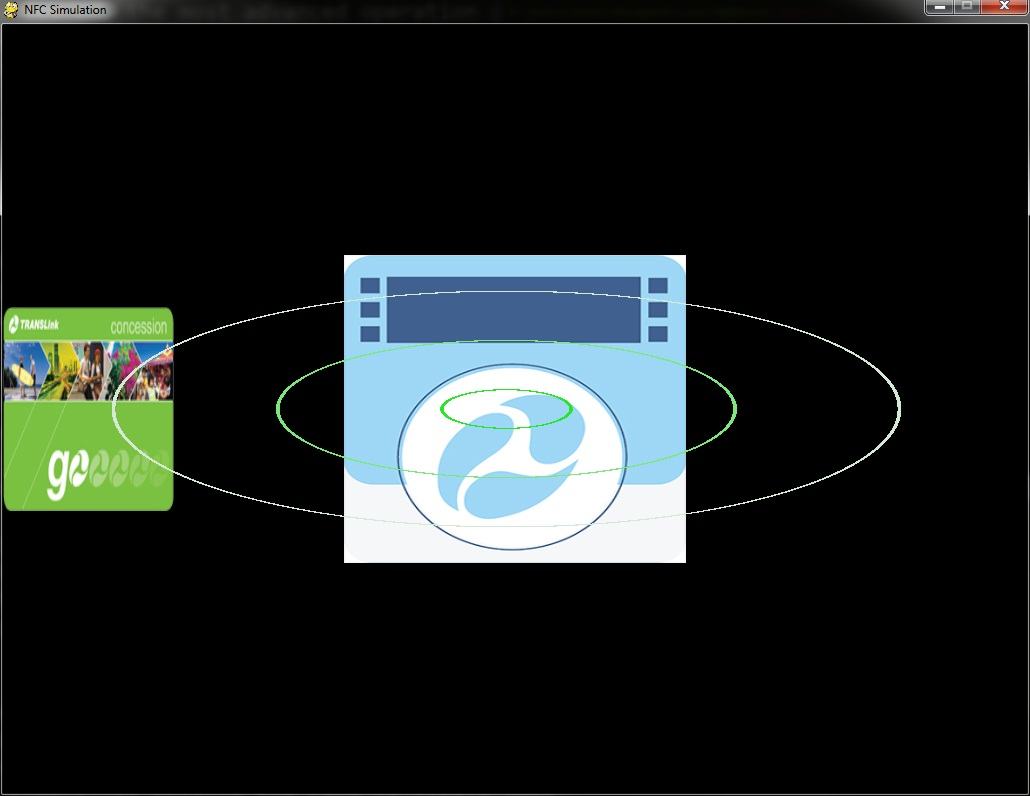
\includegraphics[width=\textwidth]{1.jpg}
    \caption{Default screen.}
  \end{minipage}
  \hfill
  \begin{minipage}[b]{0.40\textwidth}
    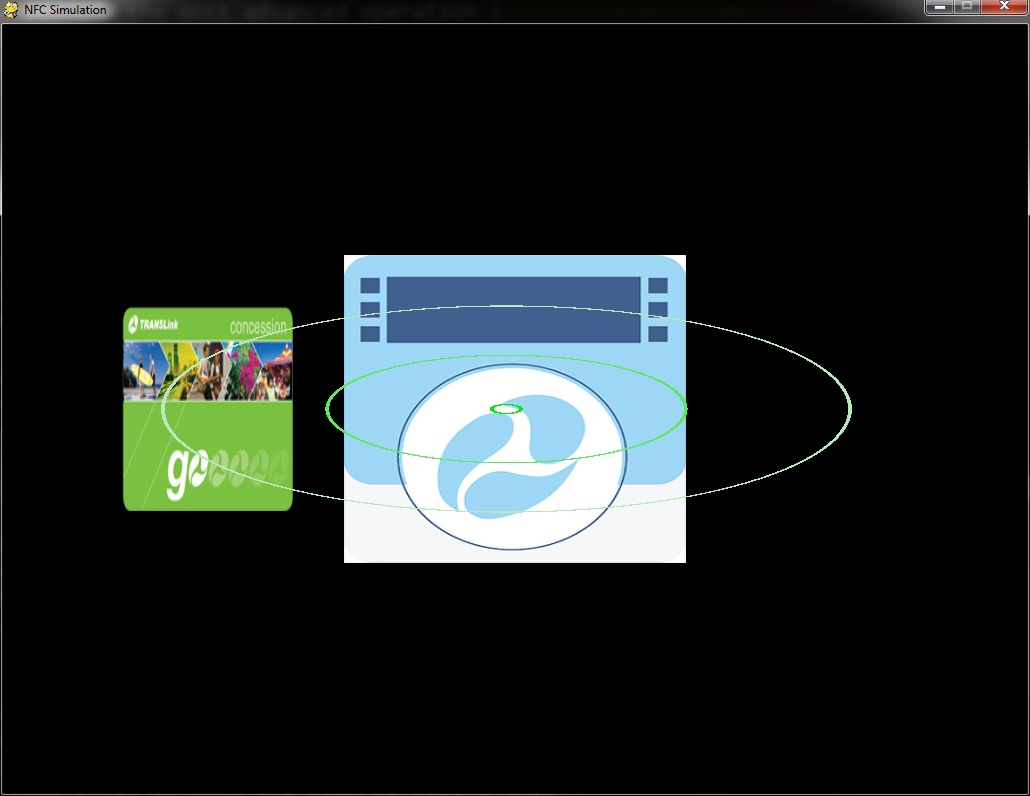
\includegraphics[width=\textwidth]{2.jpg}
    \caption{Moving the GoCard around.}
  \end{minipage}
\end{figure}

Figure 1 above is the default screen the user sees when they run the program, it depicts the GoCard on the left and the GoCard terminal in the centre of the scene (with the waves emitting from the terminal). From here, the world is the user's proverbial oyster, they have complete control, using the arrow keys, of the GoCard, and ultimately without any supervision the user will be able to discover the features of the visualization. 
Figure 2 shows the the user moving the GoCard towards the terminal using the user interaction feature. The inputs are especially easy and intuitive to use given it is using the familiar inversed T arrow keys. The WASD keys were not used as while it is familiar for gamers, the target audience are likely not as tech savvy and might intuitive go towards the directional arrow keys. The Space-bar allows the user to toggle the textures, perhaps if they would like to see the concealed antenna and tag coil. The program decides at a rate of roughly 30 times (frames) per second whether or not to redraw the textures, thus we are able to ``toggle'' which texture is drawn, depending on what the user wants. The user can exit the simulation at any time by pressing their Escape key. 

\begin{figure}[!ht]
	\centering
	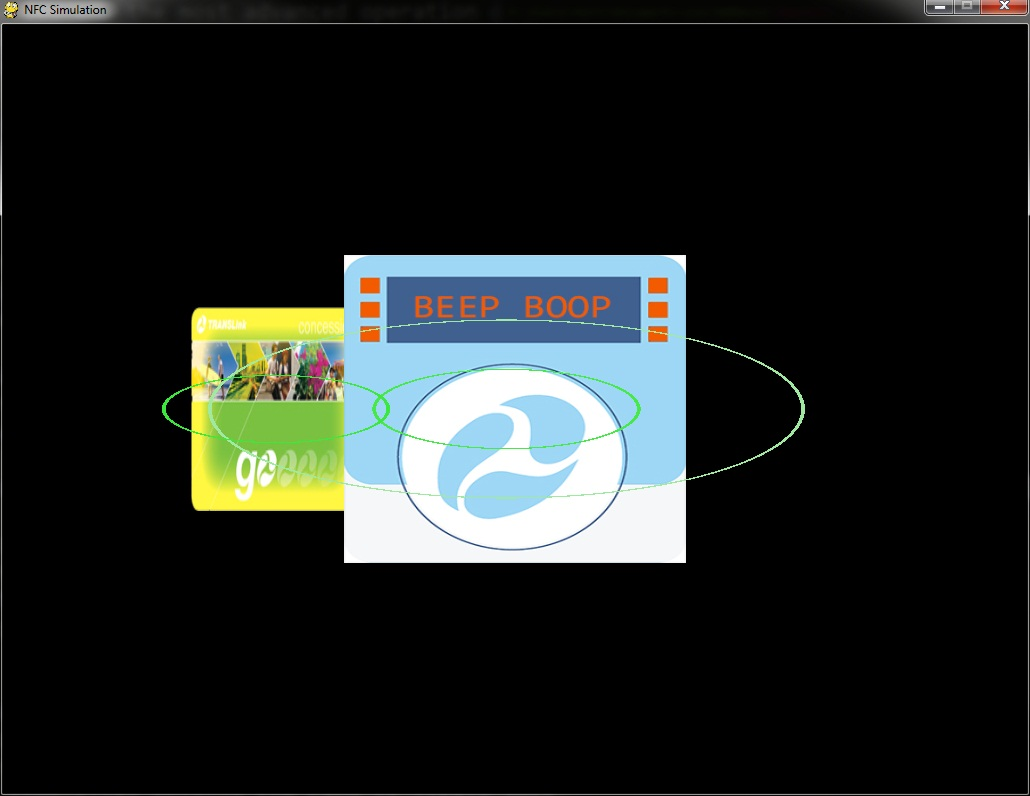
\includegraphics[scale=0.5]{3.jpg}
	\caption{Touching the GoCard on the Terminal.}
\end{figure}
Animation is the process of creating successive drawings in order to create the illusion of movement. OpenGL does not explicitly provide the means to do this, it is derived from the ability of the programmer to create logic that is capable of requesting the necessary rendering operations of the API. This project harnesses animation to simulate a simplified model of an electromagnetic field and the radiowaves necessary for Near Field Communication. Figure 3 reveals how the ``waves'' and the perspective of the scene effectively emulate a simplified model of the electromagnetic field and radio waves. By spawning a near identical new radiowave when the GoCard connects, the user can make a coherent comparison between the radiowaves emitting from the terminal and the card.

\begin{figure}[!ht]
  \centering
  \begin{minipage}[b]{0.49\textwidth}
    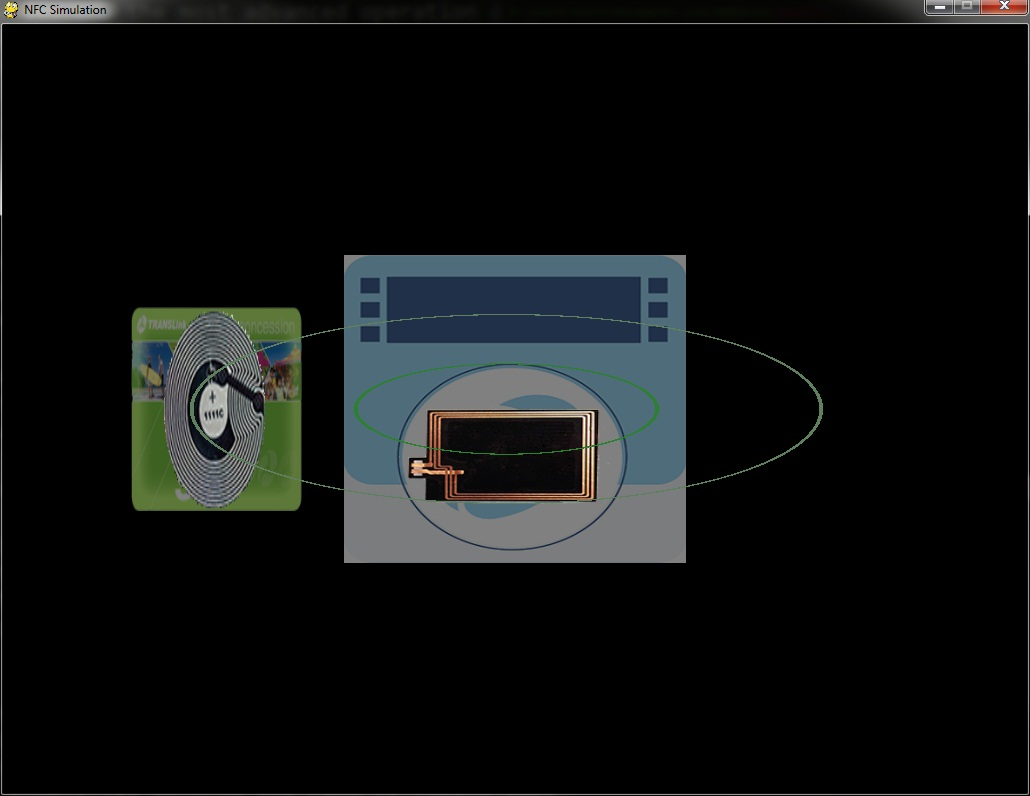
\includegraphics[width=\textwidth]{4.jpg}
    \caption{Concealed technology mode (Spacebar).}
  \end{minipage}
  \hfill
  \begin{minipage}[b]{0.49\textwidth}
    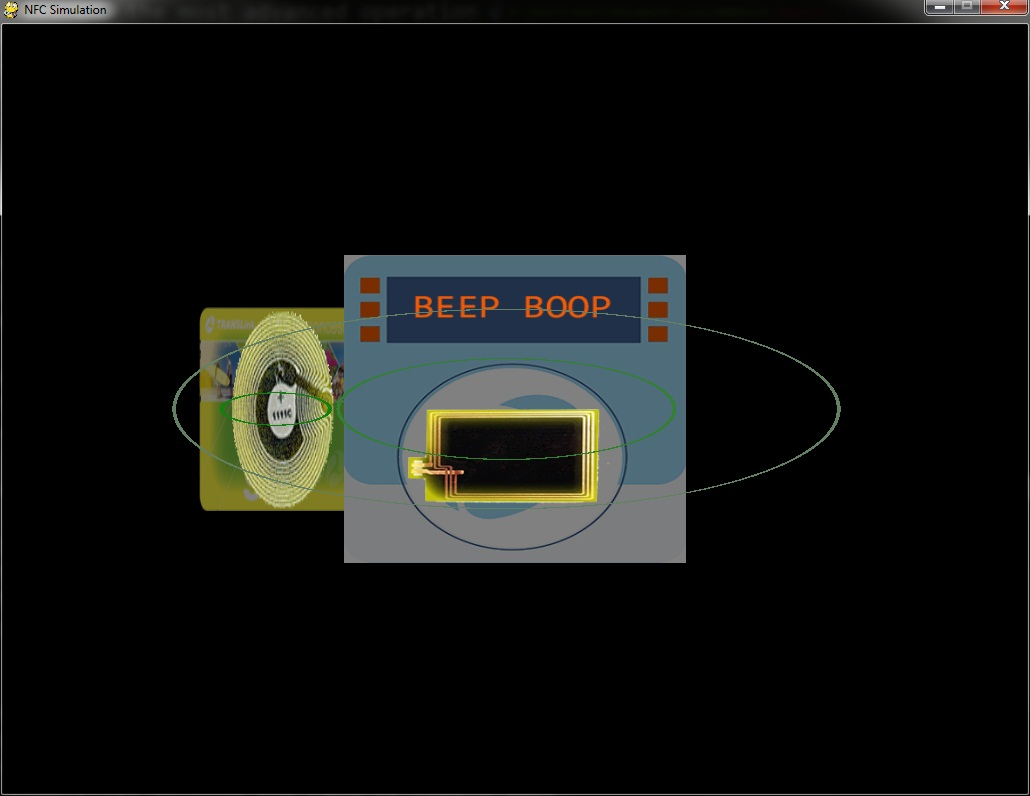
\includegraphics[width=\textwidth]{5.jpg}
    \caption{Concealed mode when touching.}
  \end{minipage}
\end{figure}

Textures are objects used by shaders and other objects to render external imagery seamlessly into an OpenGL geared program. Textures are used extensively throughout this project, particularly to complement the user's interaction. Figures 4 and 5 very effectively demonstrate this project's use of different textures to depict different states of operation and also the concealed technologies in each device. 

\section{Discussion}
In essence this project can be considered a fairly straight-forward and simple idea executed very purposefully and, somewhat, elegantly. There is a clear connection made by users between the elements. It can be said that is not as advanced or full of content however it achieves its purpose very effectively given its simple design and execution. If a user wanted to know how their GoCard works on a high level, then this computer graphics program effectively demonstrates the features of NFC. However, depending on the context / audience, it may be necessary to change the textures to something more appropriate (e.g. credit card and EFTPOS machine for financial institutions). 

The textures used to depict the GoCard and GoCard terminal perform their role well as the are responsible for relating the NFC technology to something that users are very familiar with (in this case, university students with public transport). In order to create a relatable experience it is of course important to use objects and visuals that are familiar to the users of the program. The somewhat quaint vector depiction of the GoCard terminal is especially effective as the familiarity with the machine lends itself to the complexity of the operations taking place. The use works really well because the user can relate to what is happening in the frame more so if the objects were generalized with a less specific texture. 

User interaction is a very large part of the project and given the simple controls made available to the user, this is harnessed very effectively. The ability to move the GoCard at will works very well as users seem to enjoy the freedom to play around the simulation. The GoCard lighting up and depicting a ``powered on'' state is of course scientifically inaccurate but it very effectively denotes the change in state by the card.

If someone is interested in developing a new system and at some point it may require a physical user interaction then it is likely that NFC could be broadly applied. This program through its use of animation, user interaction and texture rendering with OpenGL allows the user a glimpse at the possibilities with NFC. 

Nevertheless, the project is limited in some regards, as the underlying logic for the handling of the user interactivity could be refined. It would be helpful also to provide the user with some idea of the actual transactions taking place when two devices connect to eachother, be it very simplified or not. Whether it be the simulation of the exact bytes or not. 

\section{Conclusion}
The project set out to educate and create awareness for the NFC technology, particularly the ability to enable passive devices to become powered when in contact with an active device. 

The project looked to harness animation, texturing and user interactivity facets of computer graphics to achieve this purpose. It very effectively utilised the PyGame user input API to deliver a very simple, easy to use and intuitive program that requires no real instructions. Furthermore, the OpenGL and OpenGLU bindings made available to the Python programming language (and the CPython implementation in this instance) allowed the program to effectively draw textures to create relatability for the user. Saliently, the combination of programming logic and OpenGL's ability to draw complex shapes allowed the program to simplify the complex relationship between electromagnetic induction and NFC. 

Overall the project overcame the shortcomings as described in the discussion and should be considered an effective representation of NFC's active/passive modes of operation. 

\section{Appendices}

\subsection{Source Code}
Source is available online from the following git repository: 
\clearpage


\end{document}	